% ---------------------------------------------------
% Date:       15.05.2019
% Version:    v1.1.0
% Autor:      Felix Faltin <ffaltin91[at]gmail.com>
% Repository: https://github.com/faltfe/iodhbwm
% ---------------------------------------------------
% --- --- --- --- -- Class options -- --- --- --- ---
% ---------------------------------------------------
\documentclass[
    load-dhbw-templates,                      % Allow \dhbw* commands
    add-tocs-to-toc,                          % Add LoF, LoT, etc. to ToC
    add-bibliography,                         % Include bibliography (needs biber run)
    bib-file         = biblatex-examples.bib, % Set bibliography file
    auto-intro-pages = all,                   % Takes care about titlepage, abstract, ToC, etc.
    language         = english,               % Provide another language for the abstract
    language         = ngerman,               % Set main document language
    debug                                     % Provide \lipsum, \blindtext
]{iodhbwm}
\usepackage[T1]{fontenc}

% ---------------------------------------------------
% --- --- --- --- - Necessary setup - --- --- --- ---
% ---------------------------------------------------
\dhbwsetup{%
    abstract             = my-abstract.inc,      % Include custom abstract file
    author               = Max Mustermann,
    thesis type          = BA,
    thesis title         = Überprüfung von Bausteinen,
    student id           = 1337,
    location             = Transsilvanien,
    institute            = Lebkuchenhaus,
    institute logo       = example-image-a,
    course/id            = Txxxx,
    supervisor           = Schneewittchen,
    processing period    = {01.01.17 -- 31.01.17},
    reviewer             = Frau Holle und die sieben Zwerge,
    course/name          = {Trolltechnik},
    bachelor degree type = {Troll of the universe},
%    bachelor degree      = BoS % Bachelor of Science
}

% ---------------------------------------------------
% --- --- --- --- Begin actual content -- --- --- ---
% ---------------------------------------------------
\begin{document}

    \Blinddocument

    \chapter{Tabellen}
        \blindtext

        \begin{table}[htb]
            \centering
            \begin{tabular}{@{}ll@{}}
                \toprule
                Linke Spalte & Rechte Spalte\\\midrule
                \dots & \dots\\
                &\\
                &\\\bottomrule
            \end{tabular}
            \caption{Leere Tabelle}
        \end{table}

        \blindtext

    \chapter{Abbildungen}
        \blindtext

        \begin{figure}[htb]
            \centering
            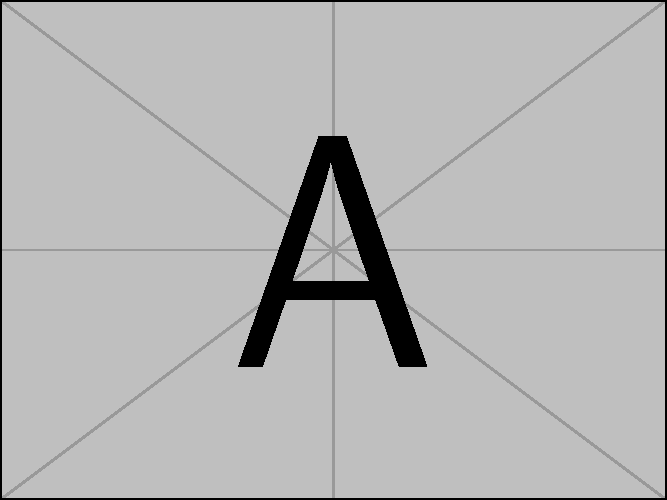
\includegraphics[width=.5\linewidth]{example-image-a}
            \caption{Random image}
        \end{figure}

        \blindtext

    % Cite all elements from the passed file
    % This is necessary because otherwise there
    % won't be any bibliography generated.
    \nocite{*}
\end{document}
